\documentclass[12pt]{report}
\usepackage[utf8]{inputenc}
\usepackage[russian]{babel}
%\usepackage[14pt]{extsizes}
\usepackage{listings}
\usepackage{graphicx}
\usepackage{amsmath,amsfonts,amssymb,amsthm,mathtools} 
\usepackage{pgfplots}
\usepackage{filecontents}
\usepackage{float}
\usepackage{comment}
\usepackage{indentfirst}
\usepackage{eucal}
\usepackage{enumitem}
%s\documentclass[openany]{book}
\frenchspacing

\usepackage{indentfirst} % Красная строка

\usetikzlibrary{datavisualization}
\usetikzlibrary{datavisualization.formats.functions}

\usepackage{amsmath}


% Для листинга кода:
\lstset{ %
	language=c,                 % выбор языка для подсветки (здесь это С)
	basicstyle=\small\sffamily, % размер и начертание шрифта для подсветки кода
	numbers=left,               % где поставить нумерацию строк (слева\справа)
	numberstyle=\tiny,           % размер шрифта для номеров строк
	stepnumber=1,                   % размер шага между двумя номерами строк
	numbersep=5pt,                % как далеко отстоят номера строк от подсвечиваемого кода
	showspaces=false,            % показывать или нет пробелы специальными отступами
	showstringspaces=false,      % показывать или нет пробелы в строках
	showtabs=false,             % показывать или нет табуляцию в строках
	frame=single,              % рисовать рамку вокруг кода
	tabsize=2,                 % размер табуляции по умолчанию равен 2 пробелам
	captionpos=t,              % позиция заголовка вверху [t] или внизу [b] 
	breaklines=true,           % автоматически переносить строки (да\нет)
	breakatwhitespace=false, % переносить строки только если есть пробел
	escapeinside={\#*}{*)}   % если нужно добавить комментарии в коде
}


\usepackage[left=2cm,right=2cm, top=2cm,bottom=2cm,bindingoffset=0cm]{geometry}
% Для измененных титулов глав:
\usepackage{titlesec, blindtext, color} % подключаем нужные пакеты
\definecolor{gray75}{gray}{0.75} % определяем цвет
\newcommand{\hsp}{\hspace{20pt}} % длина линии в 20pt
% titleformat определяет стиль
\titleformat{\section}[hang]{\Huge\bfseries}{\thechapter\hsp\textcolor{gray75}{|}\hsp}{0pt}{\Huge\bfseries}


% plot
\usepackage{pgfplots}
\usepackage{filecontents}
\usetikzlibrary{datavisualization}
\usetikzlibrary{datavisualization.formats.functions}

\begin{document}
	%\def\sectionname{} % убирает "Глава"
	\thispagestyle{empty}
	\begin{titlepage}
		\noindent \begin{minipage}{0.15\textwidth}
			
\includegraphics[width=\linewidth]{b_logo}
		\end{minipage}
		\noindent\begin{minipage}{0.9\textwidth}\centering
			\textbf{Министерство науки и высшего образования Российской Федерации}\\
			\textbf{Федеральное государственное бюджетное образовательное учреждение высшего образования}\\
			\textbf{~~~«Московский государственный технический университет имени Н.Э.~Баумана}\\
			\textbf{(национальный исследовательский университет)»}\\
			\textbf{(МГТУ им. Н.Э.~Баумана)}
		\end{minipage}
		
		\noindent\rule{18cm}{3pt}
		\newline\newline
		\noindent ФАКУЛЬТЕТ $\underline{\text{«Информатика и системы управления»}}$ \newline\newline
		\noindent КАФЕДРА $\underline{\text{«Программное обеспечение ЭВМ и информационные технологии»}}$\newline\newline\newline\newline\newline
		
		\begin{center}
			\noindent\begin{minipage}{1.1\textwidth}\centering
				\Large\textbf{Отчет по лабораторной работе №5}\newline
				\textbf{по дисциплине <<Операционные системы>>}\newline\newline
			\end{minipage}
		\end{center}
		
		\noindent\textbf{Тема} $\underline{\text{Буферизованный и не буферизованный ввод-вывод.}}$\newline\newline
		\noindent\textbf{Студент} $\underline{\text{Варламова Е. А.~~~~~~~~~~~~~~~~~~~~~~~~~~~~~~~~~~~~~~~~~~~~~~~~~~~~~~~~~~~~~~~~~}}$\newline\newline
		\noindent\textbf{Группа} $\underline{\text{ИУ7-61Б~~~~~~~~~~~~~~~~~~~~~~~~~~~~~~~~~~~~~~~~~~~~~~~~~~~~~~~~~~~~~~~~~~~~~~~~~}}$\newline\newline
		\noindent\textbf{Оценка (баллы)} $\underline{\text{~~~~~~~~~~~~~~~~~~~~~~~~~~~~~~~~~~~~~~~~~~~~~~~~~~~~~~~~~~~~~~~~~~~~~~~~}}$\newline\newline
		\noindent\textbf{Преподаватель} $\underline{\text{Рязанова Н. Ю.~~~~~~~~~~~~~~~~~~~~~~~~~~}}$\newline\newline\newline
		
		\begin{center}
			\vfill
			Москва~---~\the\year
			~г.
		\end{center}
	\end{titlepage}
\section*{Задание}
В лабораторной работе анализируется результат выполнения трех программ. Программы демонстрируют открытие одного и того же файла несколько раз. Реализация, когда файл открывается в одной программе несколько раз выбрана для простоты. Однако, как правило, такая ситуация возможна в системе, когда один и тот же файл несколько раз открывают разные процессы или потоки одного процесса. При выполнении асинхронных процессов такая ситуация является вероятной и ее надо учитывать, чтобы избежать потери данных, получения неверного результата при выводе данных в файл или чтения данных не в той последовательности, в какой предполагалось, и в результате при обработке этих данных получения неверного результата.
Каждую из приведенных программ надо выполнить в многопоточном варианте: в программах создается дополнительный поток, а работа с открываемым файлом выполняется в потоках.

Проанализировать работу приведенных программ и объяснить результаты их работы.

\section*{Программа №1}
\subsection*{Код однопоточной версии}
\begin{lstlisting}
#include <stdio.h>
#include <fcntl.h>
int main() {
    int fd = open("alphabet.txt", O_RDONLY);

    FILE *fs1 = fdopen(fd,"r");
    char buff1[20];
    setvbuf(fs1,buff1, _IOFBF, 20);

    FILE *fs2 = fdopen(fd, "r");
    char buff2[20];
    setvbuf(fs2, buff2, _IOFBF, 20);

    int flag1 = 1, flag2 = 2;

    while (flag1 == 1 || flag2 == 1) {
        char c;
        flag1 = fscanf(fs1, "%c", &c);
        if (flag1 == 1) {
            fprintf(stdout, "%c", c);
        }
        flag2 = fscanf(fs2, "%c", &c);
        if (flag2 == 1) {
            fprintf(stdout, "%c", c);
        }
    }
    return 0; }
\end{lstlisting}

\subsection*{Результат работы}
\begin{figure}[H]
	\centering
	
\includegraphics[scale=1]{res_01_one.png}
	\caption{Однопоточная версия 1-ой программы}
	\label{fig:1}
\end{figure}

\subsection*{Код многопоточной версии}
\begin{lstlisting}
#include <stdio.h>
#include <fcntl.h>
#include <pthread.h>
void thread(int fd)
{
    FILE *fs = fdopen(fd, "r");
    char buff[20];
    setvbuf(fs, buff, _IOFBF, 20);

    char c;
    int flag = fscanf(fs, "%c", &c);
    while (flag == 1) {
        fprintf(stdout, "%c", c);
        flag = fscanf(fs, "%c", &c);
    }
}
int main() {
    int fd = open("alphabet.txt", O_RDONLY);

    pthread_t tid[2];
    for (int i = 0; i < 2; i++) {
        if (pthread_create(&tid[i], NULL, thread, fd)) {
            printf("Error: can't create thread\n");
            return -1; }
    }
    pthread_join(tid[0], NULL);
    pthread_join(tid[1], NULL);
    return 0;
}
\end{lstlisting}

\subsection*{Результат работы}
\begin{figure}[H]
	\centering
	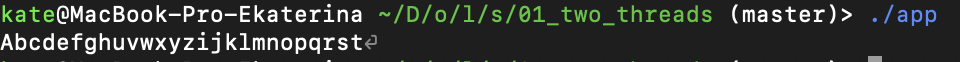
\includegraphics[scale=1]{res_01_two.png}
	\caption{Многопоточная версия 1-ой программы}
	\label{fig:1}
\end{figure}
\subsection*{Объяснение результатов}
\begin{figure}[H]
	\centering
	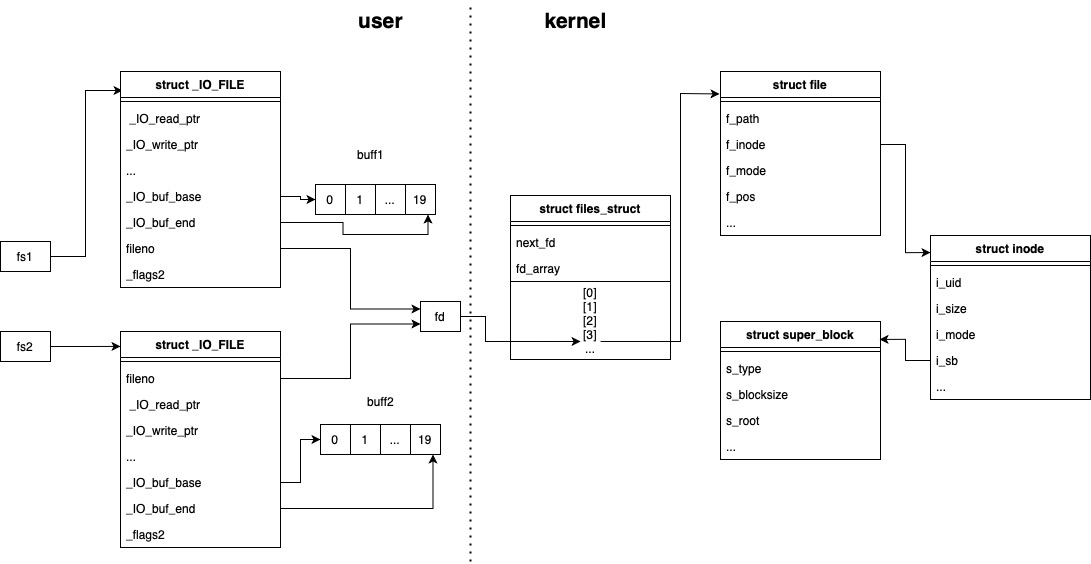
\includegraphics[scale=0.45]{os_lab_05-1.jpg}
	\caption{Связь структур}
	\label{fig:1}
\end{figure}
Системный вызов open() создаёт дескриптор открытого файла (описанного структурой struct file) и возвращает индекс в массиве fd\_array структуры files\_struct.

Вызов fdopen() создает структуры типа FILE (fs1 и fs2), которые ссылаются на дескриптор открытого файла, созданный ранее.

С помощью setbuf для структур FILE (fs1, fs2) задаются буферы и тип буферизации \_IOFBF (Fully buffered).

При первом вызове fscanf(fs1, ...) буфер структуры fs1 полностью заполнится, то есть будут прочитаны первые 20 символов, а поле f\_pos структуры struct file станет равным 20. Затем при вызове fscanf(fs2, ...) оставшиеся символы считаются в буфер структуры fs2, f\_pos структуры struct file станет равным 20 + количество оставшихся символов. При последующих вызовах fscanf(fs1, ...) и fscanf(fs2, ...) работа будет производиться с буферами, поэтому в результате будет получен приведённый результат:
\begin{itemize}
    \item в однопоточной версии вызовы fscanf(fs1, ...) и fscanf(fs2, ...) происходят поочерёдно, поэтому символы в результате соответствуют поочерёдному чтению из первого и второго буферов;
    \item в многопоточной версии порядок вызовов fscanf(fs, ...) двух потоков не определён, поэтому символы в результате соответствуют чтению из буферов в произвольном порядке.
\end{itemize}

\section*{Программа №2}
\subsection*{Код однопоточной версии}
\begin{lstlisting}
#include <stdio.h>
#include <fcntl.h>
#include <unistd.h>
int main()
{
    char c;
    int fd1 = open("alphabet.txt", O_RDONLY);
    int fd2 = open("alphabet.txt", O_RDONLY);
    int flag = 1;
    while(flag)
    {
        if (read(fd1, &c, 1) == 1) {
            write(1, &c, 1);
            if (read(fd2, &c, 1) == 1) {
                write(1, &c, 1);
            } else {
                flag = 0;
            }
        } else {
            flag = 0;
        }
    }
    return 0;
}
\end{lstlisting}

\subsection*{Результат работы}
\begin{figure}[H]
	\centering
	
\includegraphics[scale=1]{res_02_one.png}
	\caption{Однопоточная версия 2-ой программы}
	\label{fig:1}
\end{figure}
\newpage
\subsection*{Код многопоточной версии}
\begin{lstlisting}
#include <stdio.h>
#include <fcntl.h>
#include <unistd.h>
#include <pthread.h>
void thread()
{
    char c;
    int fd = open("alphabet.txt", O_RDONLY);
    while (read(fd, &c, 1) == 1)
    {
        write(1, &c, 1);
    }
}
int main()
{
    pthread_t tid[2];
    for (int i = 0; i < 2; i++) {
        if (pthread_create(&tid[i], NULL, thread, NULL)) {
            printf("Error: can't create thread\n");
            return -1; }
    }
    pthread_join(tid[0], NULL);
    pthread_join(tid[1], NULL);
    return 0;
}
\end{lstlisting}

\subsection*{Результат работы}
\begin{figure}[H]
	\centering
	
\includegraphics[scale=1]{res_02_two.png}
	\caption{Многопоточная версия 2-ой программы}
	\label{fig:1}
\end{figure}
\subsection*{Объяснение результатов}
\begin{figure}[H]
	\centering
	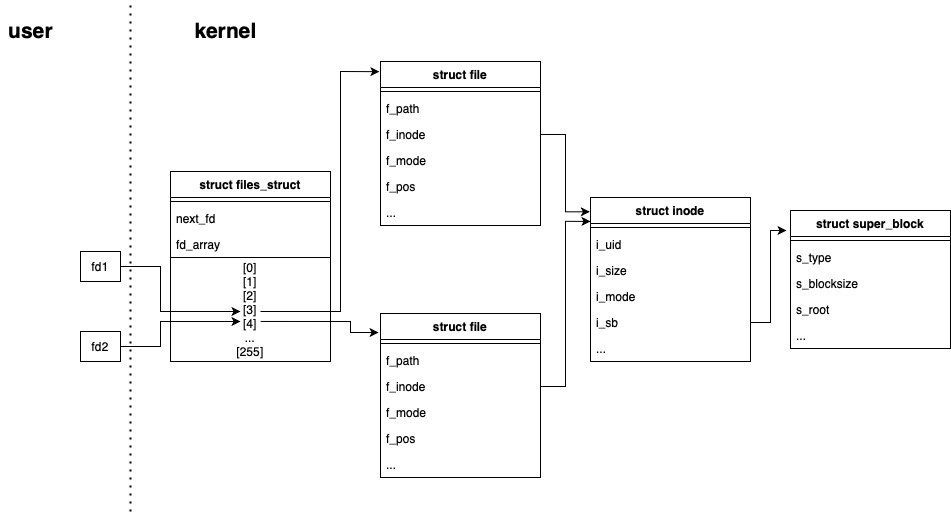
\includegraphics[scale=0.45]{os_lab_05-2.jpg}
	\caption{Связь структур}
	\label{fig:1}
\end{figure}
Системный вызов open() создаёт 2 файловых дескриптора открытого файла (описанного структурами struct file) и возвращает индекс в массиве fd\_array структуры files\_struct. Таким образом, создаётся две структуры открытого файла, каждая из которых имеет собственное поле f\_pos. Именно поэтому в результате будет получен приведённый результат:
\begin{itemize}
    \item в однопоточной версии вызовы read происходят поочерёдно, поэтому символы в результате соответствуют двум поочерёдным независимым чтениям из файла;
    \item в многопоточной версии порядок вызовов read двух потоков не определён, поэтому символы в результате соответствуют двум независимым чтениям в произвольном порядке.
\end{itemize}
\section*{Программа №3}
\subsection*{Код}
\begin{lstlisting}
#include <stdio.h>
#include <sys/stat.h>
#include <pthread.h>
#define FMT_STR " FS%d: inode = %ld, size = %ld\n"
void *thread(int data) {
    int fid = (int)data;
    struct stat statbuf;
    FILE *fs = fopen("out.txt", "w");
    stat("out.txt", &statbuf);

    printf("FOPEN " FMT_STR, fid, statbuf.st_ino, statbuf.st_size);
    for (char c = 'a'; c <= 'z'; c++) {
        if ((c % 2) == (fid == 1))
            fprintf(fs, "%c", c);
    }
    fclose(fs);
    stat("out.txt", &statbuf);
    printf("FCLOSE" FMT_STR, fid, statbuf.st_ino, statbuf.st_size);
}
int main() {
    pthread_t tid[2]; int fid[2] = {0, 1};
    for (int i = 0; i < 2; i++) {
        if (pthread_create(&tid[i], NULL, thread, fid[i])) {
            printf("Error: can't create thread\n");
            return -1; }
    }
    pthread_join(tid[0], NULL);
    pthread_join(tid[1], NULL); return 0;
}
\end{lstlisting}

\subsection*{Результат работы}
\begin{figure}[H]
	\centering
	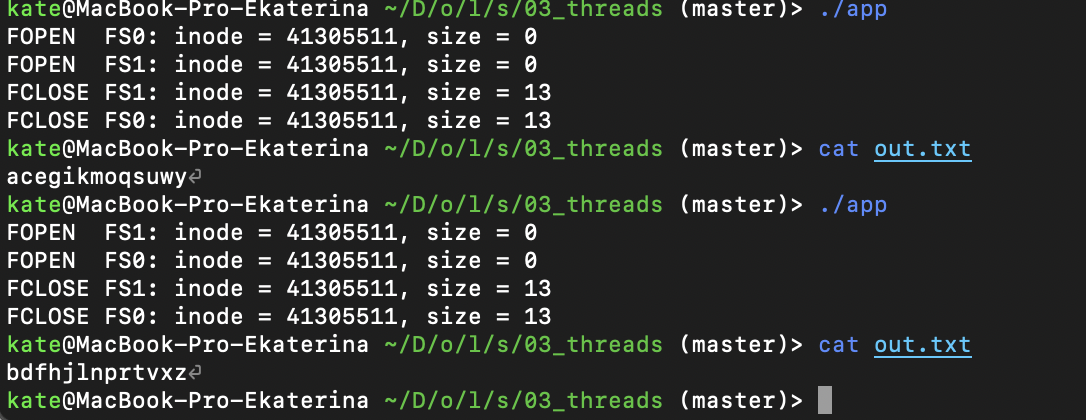
\includegraphics[scale=1]{res_03.png}
	\caption{3-я программа}
	\label{fig:1}
\end{figure}
\subsection*{Объяснение результатов}
\begin{figure}[H]
	\centering
	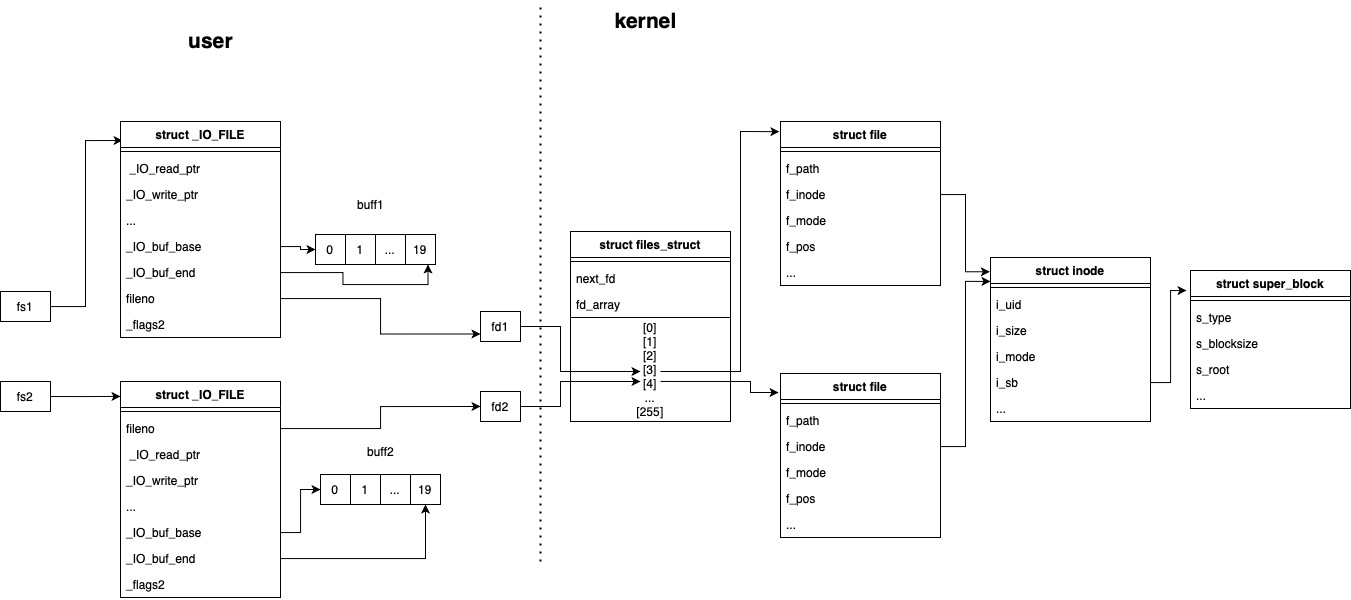
\includegraphics[scale=0.37]{os_lab_05-3.jpg}
	\caption{Связь структур}
	\label{fig:1}
\end{figure}
Вызов fopen() создаёт файловый дескриптор открытого файла (описанного структурой struct file) и возвращает индекс в массиве fd\_array структуры files\_struct. Кроме того, fopen создаёт структуру типа FILE, которая ссылается на дескриптор открытого файла, созданный ранее. Таким образом, создаётся две структуры открытого файла, каждая из которых имеет собственное поле f\_pos. 

Так как запись производится с помощью функции fprintf, использующий буферизованный ввод-вывод, то запись в двух потоках будет осуществляться в буфер. Существуют 3 условия записи из буфера в файл:
\begin{itemize}
    \item переполнение буфера;
    \item fflush;
    \item закрытие файла.
\end{itemize}

Так как буфер не переполняется и не вызывается fflush, то запись в файл в приведённой программе осуществится лишь при вызове fclose. Так как потоки работают с одним и тем же файлом, причём ссылаются на разные структуры struct file (то есть поле f\_pos для каждого потока своё), то результат записи будет зависеть от того, какой поток вызвал fclose позже. При этом данные, записанные в файл ранее, будут утеряны.

\subsection*{Решение проблемы}
Причина: каждый дескриптор открытого файла имеет своё поле f\_pos. 

\textbf{Решение №1}: необходимо использовать режим O\_APPEND. В данном режиме перемещение позиции в конец файла и добавление символа происходят атомарно, поэтому данные не будут утеряны. 

\textbf{Решение №2}: необходимо использовать мьютекс для перемещения позиции в конец файла и записи символа. Код:
\begin{lstlisting}
#include <stdio.h>
#include <sys/stat.h>
#include <pthread.h>
#include <unistd.h>

#define FMT_STR " FS%d: inode = %ld, size = %ld\n"
pthread_mutex_t lock;
void *thread(int data) {
    int fid = (int)data;
    struct stat statbuf;
    FILE *fs = fopen("out.txt", "w");
    stat("out.txt", &statbuf);

    printf("FOPEN " FMT_STR, fid, statbuf.st_ino, statbuf.st_size);
    for (char c = 'a'; c <= 'z'; c++) {
        if ((c % 2) == (fid == 1)) {
            pthread_mutex_lock(&lock);
            lseek(fileno(fs), NULL, SEEK_END);
            fprintf(fs, "%c", c);
            pthread_mutex_unlock(&lock);
        }
    }
    fclose(fs);
    stat("out.txt", &statbuf);
    printf("FCLOSE" FMT_STR, fid, statbuf.st_ino, statbuf.st_size);
}
int main() {
    if (pthread_mutex_init(&lock, NULL) != 0)
    {
        printf("\n mutex init failed\n");
        return 1;
    }
    pthread_t tid[2]; int fid[2] = {0, 1};
    for (int i = 0; i < 2; i++) {
        if (pthread_create(&tid[i], NULL, thread, fid[i])) {
            printf("Error: can't create thread\n");
            return -1; }
    }
    pthread_join(tid[0], NULL);
    pthread_join(tid[1], NULL); return 0;
}
\end{lstlisting}
\newpage
\section*{struct \_IO\_FILE}
\begin{lstlisting}
	struct _IO_FILE
	{
	  int _flags;                /* High-order word is _IO_MAGIC; rest is flags. */
	
	  /* The following pointers correspond to the C++ streambuf protocol. */
	  char *_IO_read_ptr;        /* Current read pointer */
	  char *_IO_read_end;        /* End of get area. */
	  char *_IO_read_base;        /* Start of putback+get area. */
	  char *_IO_write_base;        /* Start of put area. */
	  char *_IO_write_ptr;        /* Current put pointer. */
	  char *_IO_write_end;        /* End of put area. */
	  char *_IO_buf_base;        /* Start of reserve area. */
	  char *_IO_buf_end;        /* End of reserve area. */
	
	  /* The following fields are used to support backing up and undo. */
	  char *_IO_save_base; /* Pointer to start of non-current get area. */
	  char *_IO_backup_base;  /* Pointer to first valid character of backup area */
	  char *_IO_save_end; /* Pointer to end of non-current get area. */
	
	  struct _IO_marker *_markers;
	
	  struct _IO_FILE *_chain;
	
	  int _fileno;
	  int _flags2;
	  __off_t _old_offset; /* This used to be _offset but it's too small.  */
	
	  /* 1+column number of pbase(); 0 is unknown. */
	  unsigned short _cur_column;
	  signed char _vtable_offset;
	  char _shortbuf[1];
	
	  _IO_lock_t *_lock;
	#ifdef _IO_USE_OLD_IO_FILE
	};
	
\end{lstlisting}

\end{document}
